\documentclass[slovak]{beamer}
\usetheme{beaver}

\usepackage[T1]{fontenc}
\usepackage[utf8]{inputenc}
\usepackage{graphicx}

\newcommand{\jl}{$\frac{}{}$} 

\title{Caver XML projekt}
\date{2014}
\author{
	Jan Štourač, Henrich Lauko, Jiří Novotný, Karel Kubíček
}


\begin{document}

\begin{frame}
	\titlepage
\end{frame}

\begin{frame}
\frametitle{Caver}
	
\includegraphics[width=\linewidth]{caver_start.jpg}
\end{frame}

\begin{frame}
\frametitle{Caver}
	\begin{itemize}
		\item nástroj pre biochemikov, určený na analýzu a vizualizáciu proteínov
		\item hlavné využitie Caveru je počítanie tunelov v proteínoch
		\item vizualizačné techniky
	\end{itemize}
\end{frame}

\begin{frame}
\frametitle{Caver Application}
	\begin{center}
		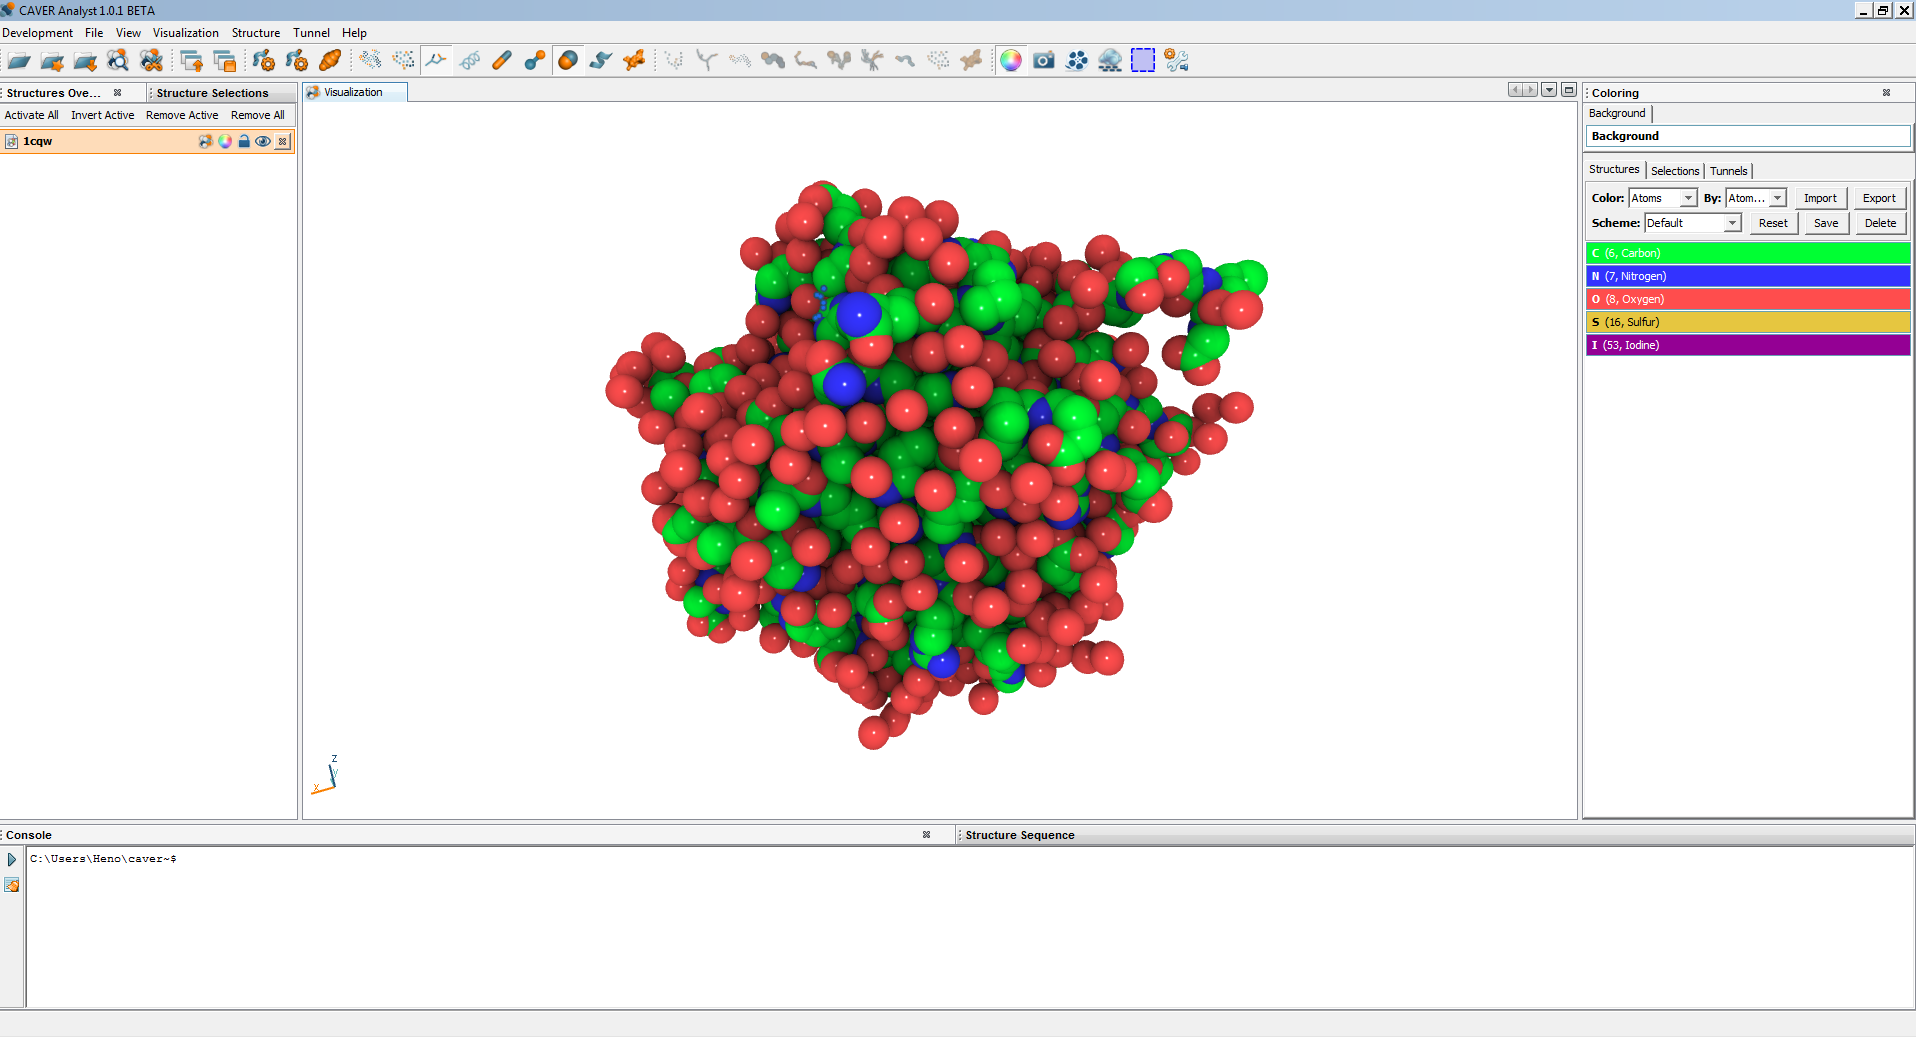
\includegraphics[width=\linewidth]{caver.png}
	\end{center}
\end{frame}



\begin{frame}
\frametitle{Ciele}
	\begin{itemize}
		\item implementovať XML do Color modulu
		\item efektívne reprezentovať farebné schémy
		\item poskytnúť uživatelom prívetive rozhranie pre prácu so svojimi schémami 
		\item úprava XML v globálnych nastaveniach Caveru
	\end{itemize}
\end{frame}

\begin{frame}
\frametitle{Organizácia projektu}
	\begin{itemize}
		\item Rozdelenie úloh:
		\begin{itemize}
			\item Color schemes backend - Jan Štourač
			\item Color schemes GUI - Henrich Lauko
			\item Color schemes XML structure and XSD - Karel Kubíček
			\item Global settings - Jiří Novotný
		\end{itemize}
		\item Práca v projektovej Caver svn
	\end{itemize}
\end{frame}

\begin{frame}
\frametitle{Proces vývoja}
	\begin{itemize}
		\item 21. 3. - stretnutie o možnostiach práce v Caveri a rozdelenie úloh
		\item 22.3. - 11.4. - zorientovanie sa v Caveri a práca na vývoji
		\item 12.4. - 20.4. - testovanie a drobné úpravy
		\item 21.4. - 27.4. - dokončovanie dokumentácie a wiki stránok
		\item 4.5. - predpokladané ukončenie práce na projekte
	\end{itemize}
\end{frame}

\begin{frame}
\frametitle{Color schémy backend}
	\begin{itemize}
		\item implementoval Jan Štourač
		\item návrh a implementácia interfacu pre prácu s farebnými schémami
		\item rozdelenie uživatelského a defaultneho rozhrania
		\item notifikácie o zmenách v schémach
	\end{itemize}
\end{frame}

\begin{frame}
\frametitle{XML color schémy}
	\begin{itemize}
		\item implementoval Karel Kubíček
		\item návrh reprezentácie farebných schém v XML
		\item rodelenie default a user schém
		\item kontrolná XSD schéma
		\item synchronizácia schém cez projektovú stránku
	\end{itemize}
\end{frame}

\begin{frame}
\frametitle{XML color GUI}
	\begin{itemize}
		\item ukazka XML / XSD (TODO obrazok)
	\end{itemize}
\end{frame}

\begin{frame}
\frametitle{Color schémy GUI}
	\begin{itemize}
		\item implementoval Henrich Lauko
		\item návrh uživatelského rozhrania
		\item rozdelenie panelov do default a user profilov
		\item riešený problém synchronizácie všetkých panelov pracujúcich s farebnými schémami
	\end{itemize}
\end{frame}

\begin{frame}
\frametitle{Color schémy GUI}
	\frametitle{Color schémy GUI}
	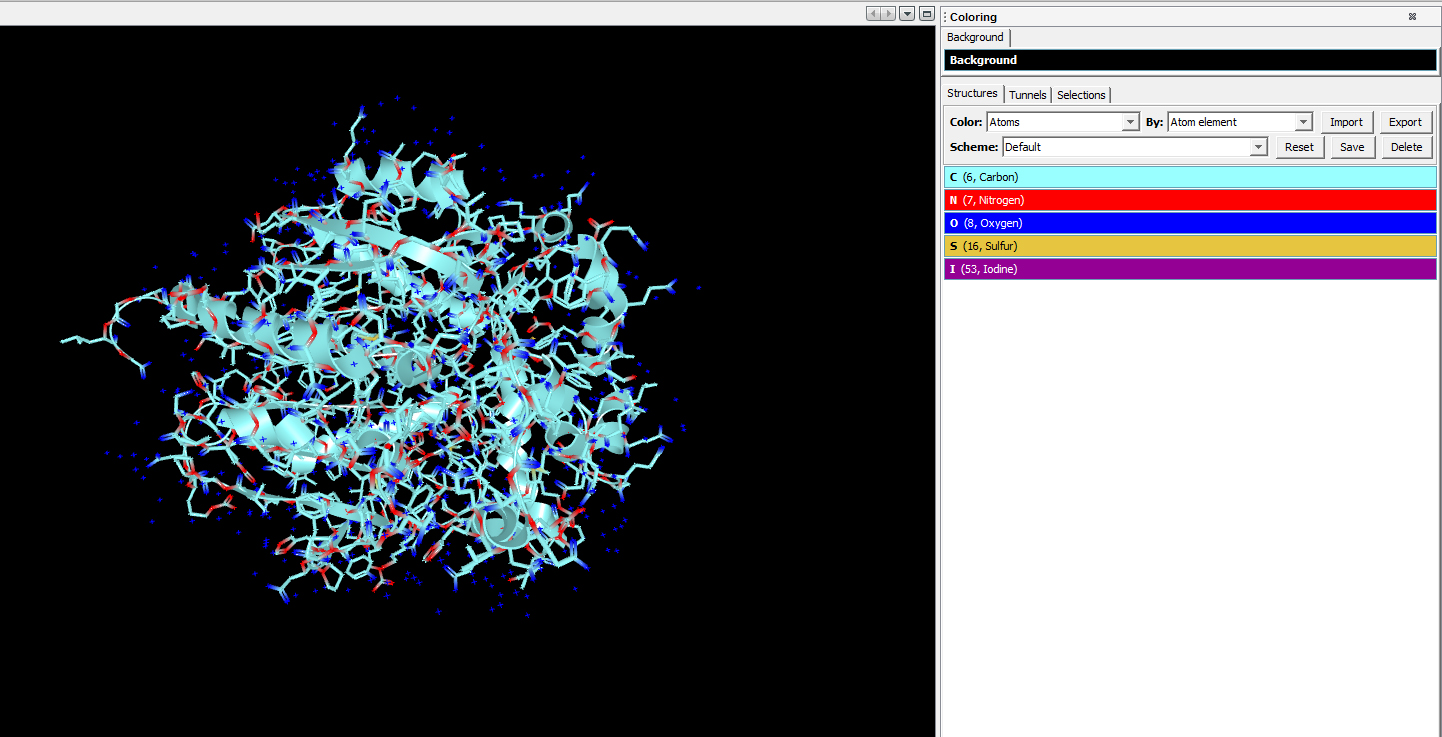
\includegraphics[width=\linewidth]{colorpanel.jpg}
\end{frame}

\begin{frame}
\frametitle{Global settings}
	\begin{itemize}
		\item Jirka slide
	\end{itemize}
\end{frame}

\begin{frame}
\frametitle{Dokumentácia projektu}
	\begin{itemize}
		\item spracovaná vo projektovej wiki Caveru
		\item prekopirované info na Git
		\item spracovaná dokumentácia do JavaDocu(písané komentáre priamo v aplikácii) a DocBooku
		\item latex prezentacia
	\end{itemize}
\end{frame}

\begin{frame}
\frametitle{Zhodnotenie vývoja}
	\begin{itemize}
		\item spracovaný funkčý Color modul s exportom a importom schém
		\item sprístupnenie zdrojového xsd na stránkach Caveru pre verejnosť na tvorbu vlastných schém
		\item zefektívnena práca medzi user a default schémami
		\item opravená práca s configurčnými súbormi
	\end{itemize}
\end{frame}

\end{document}
